% Définitions pour commencer

\begin{frame}{Graphe}
    \begin{definition}
        Un \emph{graphe orienté} est un ensemble de \emph{sommets} connectés par des emph{arcs}. Formellement, $G=(S,A)$ avec
        \begin{itemize}
            \item $S$ un ensemble de sommets 
            \item $A$ une relation binaire sur $S$ (donc une partie de $S \times S$)
        \end{itemize}
    \end{definition}

    \begin{example}
        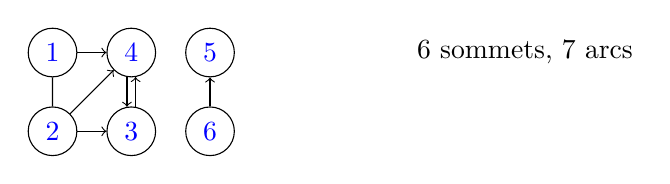
\begin{tikzpicture}
            \tikzstyle{lettre}=[circle,draw,text=blue]
            \tikzset{edge/.style = {->}}
            \node[lettre] (1) at (0,0)  {1};
            \node[lettre] (2) at (0,-1) {2};
            \node[lettre] (3) at (1,-1) {3};
            \node[lettre] (4) at (1,0) {4};
            \node[lettre] (5) at (2,0) {5};
            \node[lettre] (6) at (2,-1) {6}; 
            \node (s) at (6,0) {6 sommets, 7 arcs};
            \draw[edge] (1) -> (4);
            \draw[edge] (1) -> (2) -> (4);
            \draw[edge] (2) -> (3);
            \draw[edge] (6) -> (5);
            \draw[edge] (4.260) -> (3.100);
            \draw[edge] (3.800) -> (4.280);
        \end{tikzpicture}
    \end{example}
\end{frame}

\begin{frame}{Graphe}
    \begin{definition}
        Un \emph{graphe non orienté} est un ensemble de \emph{sommets} connectés par des emph{arêtes}. Formellement, $G=(S,A)$ avec
        \begin{itemize}
            \item $S$ un ensemble de sommets 
            \item $A$ un ensemble de paires non-ordonnées de sommets
        \end{itemize}
    \end{definition}

    \begin{example}
        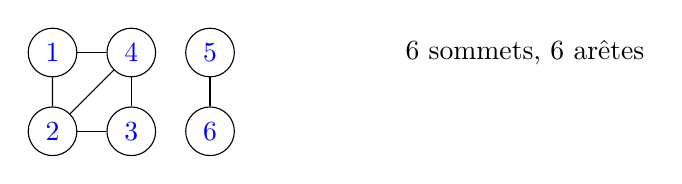
\begin{tikzpicture}
            \tikzstyle{lettre}=[circle,draw,text=blue]
            \node[lettre] (1) at (0,0)  {1};
            \node[lettre] (2) at (0,-1) {2};
            \node[lettre] (3) at (1,-1) {3};
            \node[lettre] (4) at (1,0) {4};
            \node[lettre] (5) at (2,0) {5};
            \node[lettre] (6) at (2,-1) {6}; 
            \node (s) at (6,0) {6 sommets, 6 arêtes};
            \draw (1) -- (4);
            \draw (1) -- (2) -> (4);
            \draw (2) -- (3);
            \draw (6) -- (5);
            \draw (4) -- (3);
        \end{tikzpicture}
    \end{example}
\end{frame}

\begin{frame}{Vocabulaire}
    \begin{definition}
        Dans un graphe $G(S,A)$ orienté ou non, un sommet $y$ est dit \emph{adjacent} à $x$ si et seulement si $(x,y \in A$)
    \end{definition}
    \begin{example}
        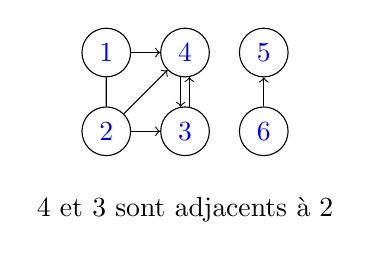
\begin{tikzpicture}
            \tikzstyle{lettre}=[circle,draw,text=blue]
            \tikzset{edge/.style = {->}}
            \node[lettre] (1) at (0,0)  {1};
            \node[lettre] (2) at (0,-1) {2};
            \node[lettre] (3) at (1,-1) {3};
            \node[lettre] (4) at (1,0) {4};
            \node[lettre] (5) at (2,0) {5};
            \node[lettre] (6) at (2,-1) {6}; 
            \draw[edge] (1) -> (4);
            \draw[edge] (1) -> (2) -> (4);
            \draw[edge] (2) -> (3);
            \draw[edge] (6) -> (5);
            \draw[edge] (4.260) -> (3.100);
            \draw[edge] (3.800) -> (4.280);
            \node (l) at (1,-2) {4 et 3 sont adjacents à 2};
        \end{tikzpicture}
        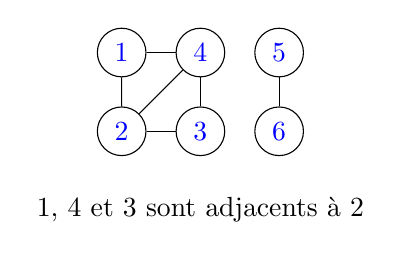
\begin{tikzpicture}
            \tikzstyle{lettre}=[circle,draw,text=blue]
            \node[lettre] (1) at (0,0)  {1};
            \node[lettre] (2) at (0,-1) {2};
            \node[lettre] (3) at (1,-1) {3};
            \node[lettre] (4) at (1,0) {4};
            \node[lettre] (5) at (2,0) {5};
            \node[lettre] (6) at (2,-1) {6}; 
            \draw (1) -- (4);
            \draw (1) -- (2) -> (4);
            \draw (2) -- (3);
            \draw (6) -- (5);
            \draw (4) -- (3);
            \node (l) at (1,-2) {1, 4 et 3 sont adjacents à 2};
        \end{tikzpicture}

    \end{example}
\end{frame}

\begin{frame}{Vocabulaire}
    \begin{definition}
        Dans un graphe $G=(S,A)$ non orienté, le degré d'un sommet est le nombre de ses sommets adjacents
    \end{definition}
    \begin{example}
        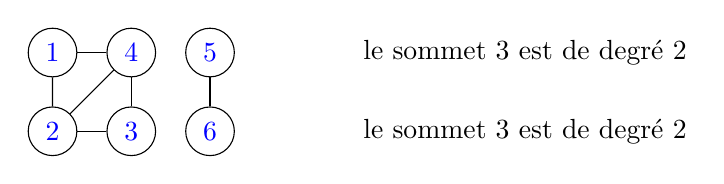
\begin{tikzpicture}
            \tikzstyle{lettre}=[circle,draw,text=blue]
            \node[lettre] (1) at (0,0)  {1};
            \node[lettre] (2) at (0,-1) {2};
            \node[lettre] (3) at (1,-1) {3};
            \node[lettre] (4) at (1,0) {4};
            \node[lettre] (5) at (2,0) {5};
            \node[lettre] (6) at (2,-1) {6}; 
            \draw (1) -- (4);
            \draw (1) -- (2) -> (4);
            \draw (2) -- (3);
            \draw (6) -- (5);
            \draw (4) -- (3);
            \node (l) at (6,0) {le sommet 3 est de degré 2};
            \node (ll) at (6,-1) {le sommet 3 est de degré 2};
        \end{tikzpicture}
    \end{example}
\end{frame}

\begin{frame}{Vocabulaire} 
    \begin{definition}
        Dans un graphe $G=(S,A)$ orienté, 
        \begin{itemize}
            \item le \emph{degré sortant} (ou extérieur) d'un sommet $x$, noté $\Gamma^+(x)$ est le nombre de ses sommets adjacents 
            \item le \emph{degré entrant} (ou intérieur) d'un sommet $x$, noté $\Gamma^-(x)$ est le nombre des sommets auxquels il est adjacent
        \end{itemize}
    \end{definition}
    \begin{example}
        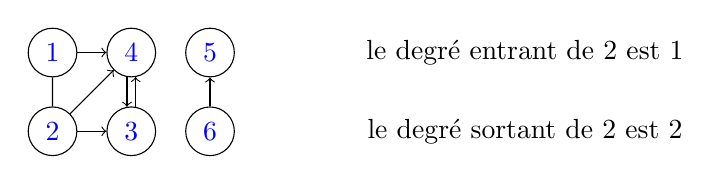
\begin{tikzpicture}
            \tikzstyle{lettre}=[circle,draw,text=blue]
            \tikzset{edge/.style = {->}}
            \node[lettre] (1) at (0,0)  {1};
            \node[lettre] (2) at (0,-1) {2};
            \node[lettre] (3) at (1,-1) {3};
            \node[lettre] (4) at (1,0) {4};
            \node[lettre] (5) at (2,0) {5};
            \node[lettre] (6) at (2,-1) {6}; 
            \draw[edge] (1) -> (4);
            \draw[edge] (1) -> (2) -> (4);
            \draw[edge] (2) -> (3);
            \draw[edge] (6) -> (5);
            \draw[edge] (4.260) -> (3.100);
            \draw[edge] (3.800) -> (4.280);
            \node (l) at (6,0) {le degré entrant de 2 est 1};
            \node (ll) at (6,-1) {le degré sortant de 2 est 2};
        \end{tikzpicture}        
    \end{example}
\end{frame}

\begin{frame}{Vocabulaire}
    \begin{definition}
        Dans un graphe $G=(S,A)$ orienté ou non, un \emph{chemin} est une suite de sommets $s_0,...s_n$ où chaque paire de sommets consécutifs $(s_k,s_{k+1})$ appartient à $a$. 
    \end{definition}
    \begin{example}
        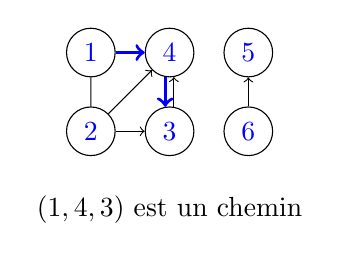
\begin{tikzpicture}
            \tikzstyle{lettre}=[circle,draw,text=blue]
            \tikzstyle{edge}=[->]
            \tikzstyle{chemin}=[->,very thick,blue]
            \node[lettre] (1) at (0,0)  {1};
            \node[lettre] (2) at (0,-1) {2};
            \node[lettre] (3) at (1,-1) {3};
            \node[lettre] (4) at (1,0) {4};
            \node[lettre] (5) at (2,0) {5};
            \node[lettre] (6) at (2,-1) {6}; 
            \draw[chemin] (1) -> (4);
            \draw[edge] (1) -> (2) -> (4);
            \draw[edge] (2) -> (3);
            \draw[edge] (6) -> (5);
            \draw[chemin] (4.260) -> (3.100);
            \draw[edge] (3.800) -> (4.280);
            \node (l) at (1,-2) {$(1,4,3)$ est un chemin};
        \end{tikzpicture}
        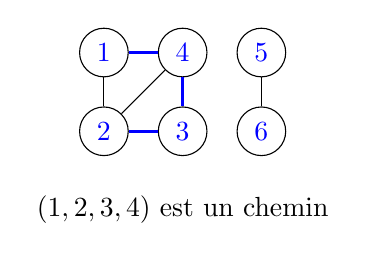
\begin{tikzpicture}
            \tikzstyle{lettre}=[circle,draw,text=blue]
            \tikzstyle{chemin}=[very thick,blue]
            \node[lettre] (1) at (0,0)  {1};
            \node[lettre] (2) at (0,-1) {2};
            \node[lettre] (3) at (1,-1) {3};
            \node[lettre] (4) at (1,0) {4};
            \node[lettre] (5) at (2,0) {5};
            \node[lettre] (6) at (2,-1) {6}; 
            \draw[chemin] (1) -- (4);
            \draw (1) -- (2);
            \draw (2) -- (4);
            \draw[chemin] (2) -- (3);
            \draw (6) -- (5);
            \draw[chemin] (4) -- (3);
            \node (l) at (1,-2) {$(1,2,3,4)$ est un chemin};
        \end{tikzpicture}
    \end{example}
\end{frame}